\entry{2026-10-19}{Priority 2: POD hyper-reduced baselines (C3) --- H-base fails}

Lane \texttt{2026-10-06-jcp-hr-baselines}, last commit \texttt{2e3abac47}, mirror \texttt{2fa5b5967}. Eleven H200 jobs, 21.18 of 30 GPU-h (three attempts cancelled after defects were found and fixed: a slow NNLS column deletion, a results-file rewrite storm, and a time-step parsing bug). Design 21 rounds, code 33, results 3 (CONFIRMED), report 5 (READY). Numbers quoted from the generated \path{report.md}. \textbf{All comparisons are developmental, in-sample and unadjusted}: both methods were tuned and compared on the same validation cases; errors are E0-conditional.

\begin{itemize}
\item \textbf{Baselines:} POD-LSPG with ECSW (support-targeted greedy NNLS) or Q-DEIM hyper-reduction, native and common solvers, POD snapshots from the central-difference FOM on the training draws.
\item \textbf{2D $1024^2$: a baseline selected by the registered role rule dominates all 8 of our qualified configurations} (faster per query and lower worst-case error, non-overlapping intervals). Like-for-like example, our R512 LSPG-CN-R: worst 2.17\,\% vs the ECSW pick's 1.35\,\% at 0.14$\times$ our time. Restriction: snapshot-limited.
\item \textbf{2D $256^2$:} 8 of 8 dominated (the saturation check failed; the registered all-step basis was used).
\item \textbf{3D $65^3$:} 7 of 9 dominated (5/5 diagnostic batch, 2/4 quadrature-qualified batch; the other 2 neutral conclusions are withheld because basis adequacy failed at ranks 768--1024). Most frequent pick: ECSW $r=512$, $\kappa=8$, BDF2 at $\Delta t=1/60$ --- a different scheme and step from ours, so basis, hyper-reduction and solver effects are not separated.
\item \textbf{Caveats:} median error sometimes reverses (e.g.\ 3D W256: ours 0.57\,\% vs pick 1.11\,\%). Tuning budget: 2D unresolved against the factor-1.25 band (baseline/ours 1.16--1.73); 3D the baseline spent less (0.51--0.66).
\item Coordinator cross-check: the lane's ``ours'' errors equal priority 1's independent export (R512 CN-R worst 0.02167 at $1024^2$).
\end{itemize}
\begin{center}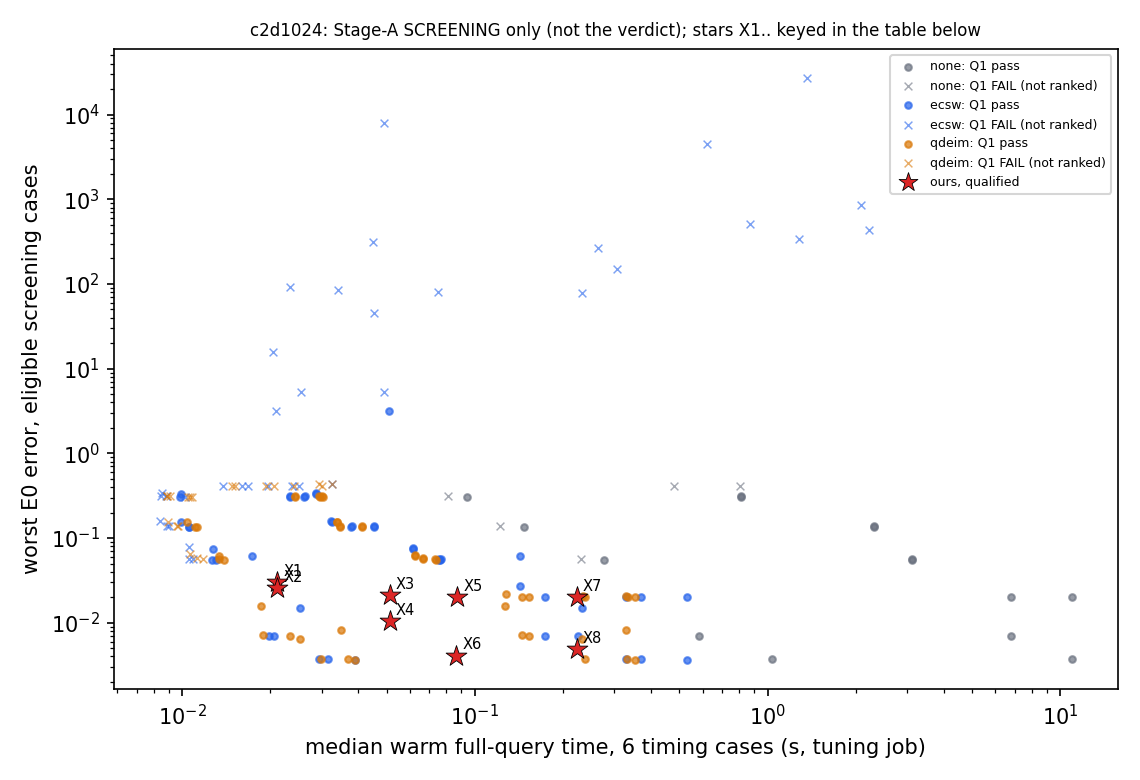
\includegraphics[width=0.48\linewidth]{figs/c3_front_2d1024.png}\hfill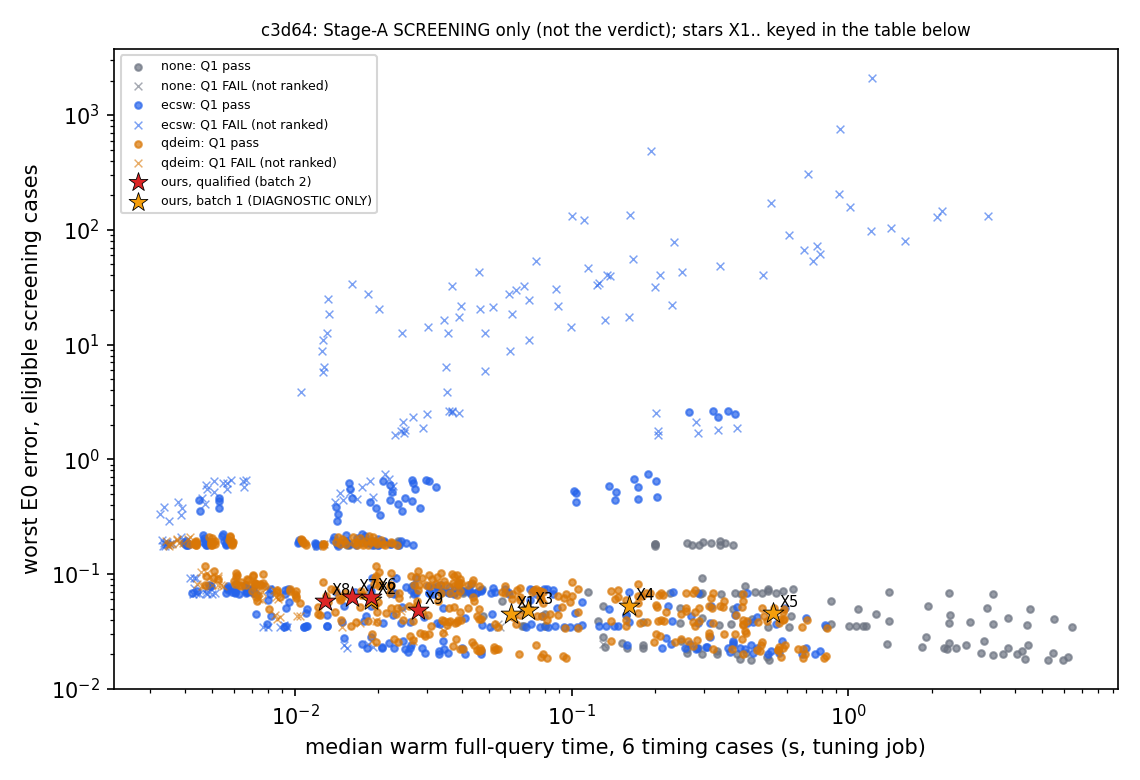
\includegraphics[width=0.48\linewidth]{figs/c3_front_3d64.png}\end{center}

\subsection*{Consequence}
H-base (``matches or beats POD-based hyper-reduced ROMs at equal tuning budget'') \textbf{fails} on this developmental evidence: a standard POD+ECSW/Q-DEIM model is faster and more accurate in the worst case on the box. With K2 also firing in both dimensions, the method's remaining distinctive claims are mesh-independent cost and mesh-free evaluation; speed and accuracy advantages over standard alternatives are not supported for viscous Burgers on the box.
